\documentclass[a4paper,12pt, oneside]{book}

%\usepackage{fullpage}
\usepackage[italian]{babel}
\usepackage[utf8]{inputenc}
\usepackage{amssymb}
\usepackage{amsthm}
\usepackage{graphics}
\usepackage{amsfonts}
\usepackage{listings}
\usepackage{amsmath}
\usepackage{amstext}
\usepackage{engrec}
\usepackage{rotating}
\usepackage[safe,extra]{tipa}
\usepackage{showkeys}
\usepackage{multirow}
\usepackage{hyperref}
\usepackage{microtype}
\usepackage{enumerate}
\usepackage{braket}
\usepackage{marginnote}
\usepackage{pgfplots}
\usepackage{cancel}
\usepackage{polynom}
\usepackage{booktabs}
\usepackage{enumitem}
\usepackage{framed}
\usepackage{pdfpages}
\usepackage{pgfplots}
\usepackage[cache=false]{minted}
\usepackage{fancyhdr}
\pagestyle{fancy}
\fancyhead[LE,RO]{\slshape \rightmark}
\fancyhead[LO,RE]{\slshape \leftmark}
\fancyfoot[C]{\thepage}



\title{Sistemi distribuiti}
\author{UniShare\\\\Davide Cozzi\\\href{https://t.me/dlcgold}{@dlcgold}\\\\Gabriele De Rosa\\\href{https://t.me/derogab}{@derogab} \\\\Federica Di Lauro\\\href{https://t.me/f_dila}{@f\textunderscore dila}}
\date{}

\pgfplotsset{compat=1.13}
\begin{document}
\maketitle

\definecolor{shadecolor}{gray}{0.80}

\newtheorem{teorema}{Teorema}
\newtheorem{definizione}{Definizione}
\newtheorem{esempio}{Esempio}
\newtheorem{corollario}{Corollario}
\newtheorem{lemma}{Lemma}
\newtheorem{osservazione}{Osservazione}
\newtheorem{nota}{Nota}
\newtheorem{esercizio}{Esercizio}
\tableofcontents
\renewcommand{\chaptermark}[1]{%
\markboth{\chaptername
\ \thechapter.\ #1}{}}
\renewcommand{\sectionmark}[1]{\markright{\thesection.\ #1}}
\chapter{Introduzione}
\textbf{Questi appunti sono presi a le lezioni. Per quanto sia stata fatta una revisione è altamente probabile (praticamente certo) che possano contenere errori, sia di stampa che di vero e proprio contenuto. Per eventuali proposte di correzione effettuare una pull request. Link: } \url{https://github.com/dlcgold/Appunti}.\\
\textbf{Grazie mille e buono studio!}
\chapter{Introduzione ai Sistemi Distribuiti}
\textit{Un sistema distribuito è un sistema nel quale componenti hardware e software, collocati in computer connessi alla rete, comunicano e coordinano le loro azione solitamente col passaggio di messaggi (a differenza delle chiamate di procedura che si hanno col passaggio di parametri su memoria condivisa)}. Ogni processo ha quindi una parte di logica applicativa e una parte di coordinamento. Altrimenti si ha questa definizione. \textit{un sistema distribuito è un insieme di elementi autonomi di computazione che si interfacciano agli utenti come un singolo sistema "coerente"}.
\begin{center}
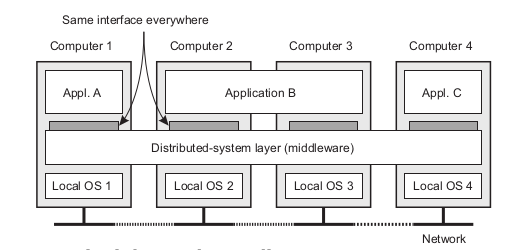
\includegraphics[scale=2.5]{img/cli.png}
\end{center}
I sistemi distribuiti sono quindi sistemi complessi. Si hanno le seguenti caratteristiche:
\begin{itemize}
\item le unità autonome di computazione si chiamano \textbf{nodi} e possono essere device hardware o singoli processi software
\item ogni nodo "fa quello che vuole", ogni nodo è autonomo, e vanno tra loro sincronizzati e coordinati (programmazione concorrente). Ogni nodo ha la sua "nozione di tempo"
\item utenti e applicazioni vedono un singolo sistema
\item si possono aprire e chiudere gruppi di nodi
\end{itemize}
La parola chiave è \textbf{trasparenza di distribuzione (distribution trasparency)}. Trasparenza significa nascondere dettagli agli utenti che possono ignorare ciò che succede e che non possono modificare il servizio. Si ha che il sistema non va in errore se un solo nodo va in errore in quanto i nodi sono indipendenti ma è difficile occultare gli errori parziali dei singoli nodi ed è difficile sistemare gli eventuali errori del singolo nodo. Ovviamente non si ha memoria condivisa e non c'è uno stato globale. In un sistema distribuito non si ha un clock globale e non si può controllare globalmente o avere uno scheduling globale.
\subsection{Il modello Client-Server}
\begin{center}
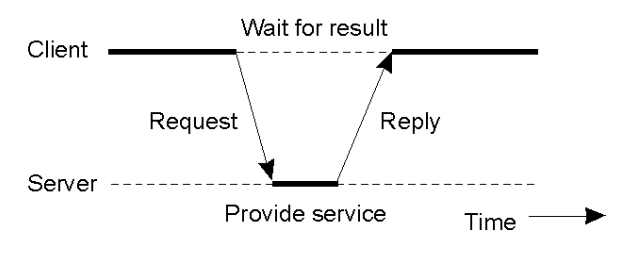
\includegraphics[scale=0.6]{img/cli2.png}
\end{center}
Si ha che un client fa una richiesta e il server risponde con un certo risultato (con il conseguente ritardo, a differenza del modello a chiamata di procedura).  
\begin{center}
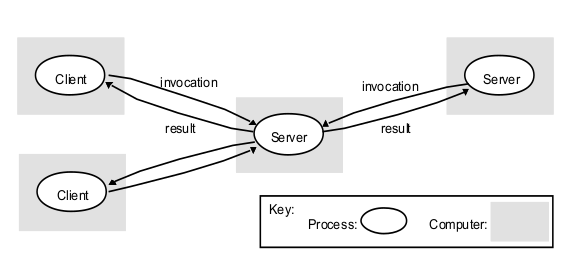
\includegraphics[scale=2.6]{img/cli3.png}
\end{center}
Si può accedere a server multipli (cluster con anche bilanciamento del carico) e si può accedere via proxy (dei server "finti" che fungono da concentratori).\\
Un sistema distribuito ha 4 problemi da fronteggiare:
\begin{enumerate}
\item \textbf{identificare la controparte}, che si risolve assegnando un nome, è la procedura di \textbf{naming}
\item \textbf{accedere alla controparte}, che si risolve con una reference, un \textbf{access point}
\item \textbf{comunicare (parte 1)}, che si risolve accettando e condividendo un formato, un \textbf{protocollo, "protocol"}
\item \textbf{comunicare (parte 2)}, che si risolve concordando \textit{sintassi e semantica} per l'informazione da condividere \textbf{(quest'ultimo è però ancora un problema aperto)}
\end{enumerate}
Si hanno le seguenti definizioni per quanto riguarda la trasparenza:
\begin{itemize}
\item \textbf{naming}, usare nomi simbolici per identificare le risorse che sono parte del sistema distribuito
\item \textbf{access trasparency}, nascondere le differenze nella rappresentazione delle informazioni e nell'accedere ad un'informazione locale o remota 
\item \textbf{location trasparency}, nascondere dove è collocata una risorsa sulla rete
\item  \textbf{relocation or mobility transparency}, nascondere che una risorsa può essere stata trasferita ad un'altra locazione mentre è in uso
\item \textbf{migration trasparency}, nascondere che una risorsa può essere trasferita
\item \textbf{replication transparency}, nascondere che una risorsa può essere replicata
\item \textbf{concurrency transparency}, nascondere che una risorsa può essere condivisa da molti utenti indipendenti
\item \textbf{failure trasparency}, nascondere fallimenti e recovery di una risorsa
\item \textbf{persistence trasparency}, nascondere se una risorsa è volatrile o memorizzata permanentemente
\end{itemize}
non si possono però nascondere:
\begin{itemize}
\item \textbf{ritardi e latenze di comunicazione}
\item \textbf{nascondere completamente i failure della rete e dei nodi}, non puoi neanche distinguere bene rallentamenti e errori. Ovviamente non puoi sapere se sta per accadere un \textbf{crash}
\end{itemize}
Una trasparenza completa, oltre ad essere quasi impossibile a livello teorico, è anche estremamente "cara" a livello di performances e tempistiche (causa scrittura costante su dischi e mantenimento delle repliche).\\
Nascondere le informazioni è alla base dell'ingegneria del software. Bisogna separare il \textit{cosa} si fa e il \textit{come} lo si fa. Il \textit{cosa} si fa mediante la definizione dell'interfaccia, \textit{Interface Definition Languages (IDL)}, e il \textit{come} mediante l'implementazione delle classi e dei metodi. Le interfacce sono definite mediante principi standard, sono complete e sono neutrali (indipendenti dall'implementazione).
\begin{center}
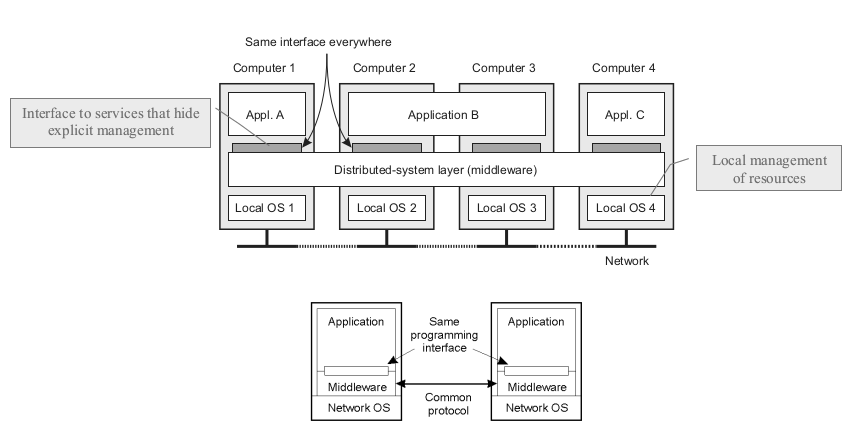
\includegraphics[scale=2]{img/cli4.png}
\end{center}
Tra i vari componenti si ha:
\begin{itemize}
\item \textbf{indipendenza logica}, con i vari componenti che lavorano autonomamente
\item \textbf{composizione}, con la collaborazione dei vari processi
\end{itemize}
Si separano:
\begin{itemize}
\item \textbf{meccanismi}, ciò che è fatto dai componenti (esempio il context switch)
\item \textbf{politiche}, come vengono applicati le varie funzionalità del sistema (esempio lo scheduling Round Robin RR)
\end{itemize}
Bisogna separare e bilanciare politiche e meccanismi
\begin{center}
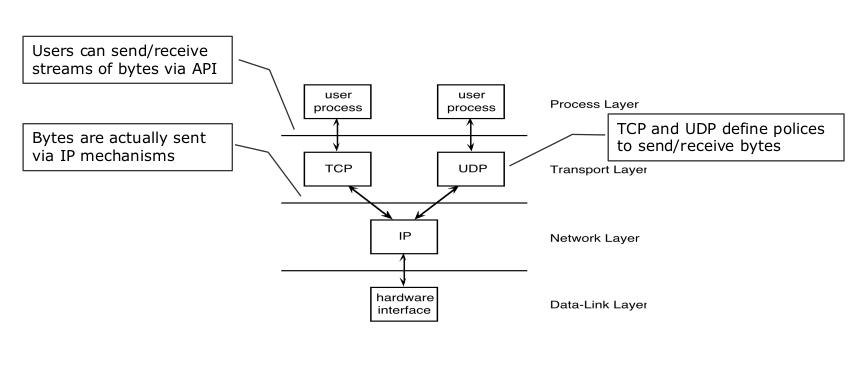
\includegraphics[scale=2]{img/cli5.png}
\end{center}
Ricapitolando il concetto di protocollo:
\begin{itemize}
\item per poter capire le richieste e formulare le risposte i due processi devono concordare un protocollo
\item i protocolli (come \textit{HTTP, FTP e SMTP}) definiscono il formato, l'ordine di invio e di ricezione dei messaggi tra i dispositivi, il tipo dei dati e le azioni da eseguire quando si riceve un messaggio
\item le applicazioni su TCP/IP:
\begin{itemize}
\item si scambiano stream di byte di lunghezza infinita (il meccanismo)
\item che possono essere segmentati in messaggi (la politica) definiti da un protocollo condiviso
\end{itemize}
\end{itemize}
Vediamo un esempio di codice. Partiamo dall'\textit{header.h}
\begin{minted}{c}
// definizioni necessarie a client e server 

#define TRUE 1
#define MAX_PATH 255 // lunghezza massima del nome di un file
#define BUF_SIZE 1024 // massima grandezza file trasferibili per volta
#define FILE_SERVER 243 // indirizzo di rete del file del server

// operazioni permesse 

#define CREATE 1 // crea un nuovo file
#define READ 2 // legge il contenuto di un file e lo restituisce
#define WRITE 3 // scrive su un file
#define DELETE 4 // cancella un file

// errori

#define OK 0 // nessun errore
#define E_BAD_OPCODE -1 // operazione sconosciuta
#define E_BAD_PARAM -2 // errore in un parametro
#define E_IO -3 // errore del disco o errore di I/O

// definizione del messaggio

struct message{
  long source; // identità del mittente
  long dest; // identità del ricevente
  long opcode; // operazione richiesta
  long count; // numero di byte da trasferire
  long offset; // posizione sul file da cui far partire l'I/O
  long result; // risultato dell'operazione
  char name[MAX_PATH]; // nome del file
  char data[BUF_SIZE]; //informazione da leggere o scrivere
};
\end{minted}
\newpage
vediamo la struttura di un semplice server che realizza un semplice file server remoto:
\begin{minted}{c}
#include <header.h>
void main(void){
  struct message m1, m2; // messaggio in entrata e uscita
  int r; // risultato
  
  while(TRUE){ // il server è sempre in esecuzione
    receive(FILE_SERVER, &m1); // stato di wait in attesa di m1
    switch(m1.code){ // vari casi in base alla richiesta
      case CREATE: 
        r = do_create(&m1, &m2);
        break;
      case CREATE: 
        r = do_read(&m1, &m2);
        break;
      case CREATE: 
        r = do_write(&m1, &m2);
        break;
      case CREATE: 
        r = do_delete(&m1, &m2);
        break;
      default:
        r = E_BAD_OPCODE;
    }
    
    m2.result = r; // ritorna il risultato al client
    send(m1.source, &m2); // manda la risposta
    
  }
}  
\end{minted}
\newpage
vediamo ora un client che usa il servizio per straferire un file:
\begin{minted}{c}
#include <header.h>

int copy(char *src, char *dst){ // copia file usando il server
  strcut message m1; // buffer del messaggio
  long position; // attuale posizione del file
  long client = 110; // indirizzo del client
  
  initialize(); // prepara l'esecuzione
  position = 0; 
  do{
    m1.opcode = READ; // operazione settata su READ
    m1.offset = position; // scelta la posizione nel file
    m1.count = BUF_SIZE; // byte da leggere
    strcpy(&m1.name, src); // nome file copiato in m1
    send(FILESERVER, &m1); // manda il messaggio al file server
    receive(client, &m1); // aspetta la risposta
    
    // scrive quanto ricevuto su un file di destinazione
    m1.opcode = WRITE; // operazione settata su WRITE
    m1.offset = position; // scelta la posizione nel file
    m1.count = BUF_SIZE; // byte da leggere
    strcpy(&m1.name, dst); // nome del file sul buffer
    send(FILESERVER, &m1); // manda il messaggio al file server
    receive(client, &m1); // aspetta la risposta
    position += m1.result // il risultato sono i byte scritti
  }while(m1.result > 0); // itera fino alla fine
  return(m1.result >= 0 ? OK : m1.result); // ritorna OK o l'errore
}

\end{minted}
\subsection{Stream Communication}
\begin{center}
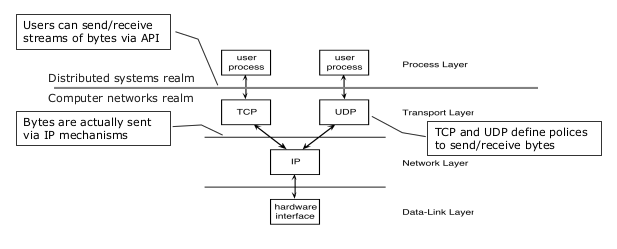
\includegraphics[scale=2.5]{img/sc.png}
\end{center}
Si ha il modello ISO/OSI, che si basa sull'astrazione. Un informatico dovrebbe conoscere tutti i vari livelli. Gli utenti possono mandare e ricevere stream di byte via TCP mediante API. Poi al livello successivo si hanno datagrammi con i dati che vengono mandai via meccanismi IP. È lo sviluppatore a decidere le varie politiche. I sistemi distribuiti lavorano tra utenti e TCP/UDP. Ovviamente sono i processi che comunicano tra di loro. Ogni processo comunica attraverso canali. Un canale gestisce i flussi di dati in ingresso e uscita e dall'esterno ogni canale è identificato da un intero detto \textbf{porta}. Le \textbf{socket} sono particolari canali per la comunicazione tra processi che non condividono memoria (per esempio perché risiedono su macchine diverse). Per potersi connettere o inviare dati ad un processo A, un processo B deve conoscere la macchina (host) che esegue A e la porta cui A è connesso (well-known port).   TCP è orientato alla connessione (si ha un invio di richiesta di connessione), è affidabile, si ha un controllo di flusso, si ha un controllo della congestione ma non si hanno garanzie di banda e ritardo minimi. UDP non è affidabile e non offre nulla di quanto offerto da TCP ma è comodo, per esempio, nello streaming, che tollera perdite parziali. UDP scompone i messaggi in pacchetti che invia uno per volta ai servizi network. TCP scompone e invia come UDP ma ogni pacchetto viene numerato per garantire riordinamento, duplicazioni e perdite. Nei sistemi distribuiti non è necessario conoscere tutto questo funzionamento ma importa solo lo stream di byte. TCP utilizza variabili e buffer per realizzare il trasferimenti bidirezionale di flussi di bytes (“pipe”) tra processi, prevede ruoli client/server durante la connessione ma non durante la comunicazione. TCP utilizza i servizi dello strato IP per l'invio dei flussi di bytes.\\
L'interfaccia tra applicazione e strato di trasporto è dato delle API, \textit{Application Programming Interface}  e i socker sono API per accedere a TCP o UDP, due processi comunicano mediante socker nel modello client-server.\\
Si hanno delle criticità:
\begin{itemize}
\item gestione del ciclo di vita di cliente e server, attivazione/terminazione del cliente e del server
\item identificazione e accesso al server
\item comunicazione tra client e server
\item ripartizione dei compiti tra client e server, che dipende dal tipo di applicazioni e la scelta influenza le prestazioni in relazione al carico
\end{itemize}
l'indirizzo del server può essere una costante nel codice, può essere chiesto all'utente, come nel browser, posso usare un nameserver o un repository (con DNS, \textit{Domain Name Service}) o adottare altri protocolli, come DHCP. Il naming sarà il nome dell'host, l'indirizzo IP come access point mediante host e porta, il protocollo saranno stream di byte e la sintassi e la semantica saranno definiti dall'applicazione con http, smtp etc...\\
Tutto questo è a un basso livello di trasparenza in quanto sia utente che sviluppatore lo necessitano.\\
La comunicazione TCP/IP avviene attraverso flussi di byte
(byte stream), dopo una connessione esplicita, tramite
normali system call read/write. Queste due syscall sono sospensive (mettono il sistema in uno stato di \textit{wait}) e usano un buffer per garantire flessibilità (per esempio la read definisce un buffer per leggere N caratteri, ma potrebbe ritornare avendone letti solo k<N)
\begin{center}
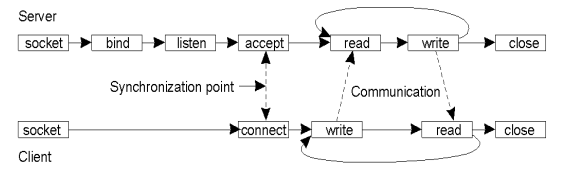
\includegraphics[scale=0.7]{img/sc2.png}
\end{center}
\newpage
Ci sono molte chiamate diverse per accedere i servizi TCP e UDP:
\begin{center}
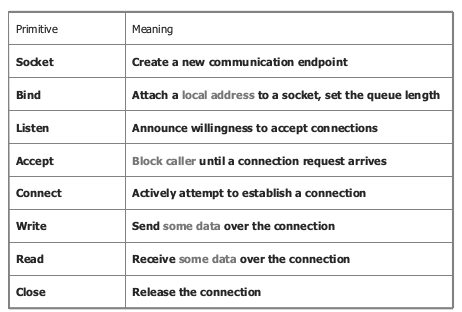
\includegraphics[scale=3]{img/sc3.png}
\end{center}

Il server crea una nuova socket collegata (binded) a una
nuova porta per comunicare con il client, in questo modo la well-known port resta dedicata a ricevere richieste di connessione:
\begin{center}
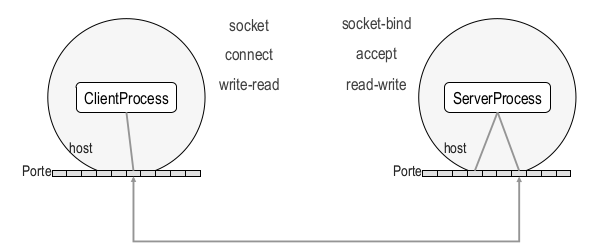
\includegraphics[scale=3]{img/sc4.png}
\end{center}
Non uso la stessa porta per evitare perché comunicazione e handshake non sarebbero distinguibili\\
Quando si parla di socket non c'è il concetto di messaggio e read/write avvengono per un numero arbitrario di bytes. Quindi si devono prevedere cicli di lettura che
termineranno in base alla dimensione dei “messaggi” come
stabilito dal formato del protocollo applicativo in uso. \\
Il prototipo della read in pseudocodice sarebbe:
\begin{minted}{c}
byteLetti read(socket, buffer, dimBuffer);
\end{minted}
con:
\begin{itemize}
\item byteLetti = byte effettivamente letti
\item socket = canale da cui leggere
\item buffer = sapzio di memoria dove trasferire i byte letti
\item dimBuffer = dimensione del buffer = numero max di caratteri che si possono leggere
\end{itemize}
\textbf{Quindi si devono prevedere cicli di lettura che
termineranno in base alla dimensione dei “messaggi” come
stabilito dal formato del protocollo applicativo in uso}\\
Java definisce alcune classi che costituiscono un'interfaccia ad oggetti alle system call:
\begin{minted}{java}
java.net.Socket
java.net.ServerSocket
\end{minted}
Queste classi accorpano funzionalità e mascherano alcuni
dettagli con il vantaggio di semplificarne l'uso.
Come per ogni framework è necessario conoscerne il modello
e il funzionamento per poterlo utilizzare in modo efficace.
Le prossime slide discutono i principali metodi delle due classi. vediamo altro, iniziamo dai costruttori:
\begin{minted}{java}
public Socket()
// Creates an unconnected socket, with the system-default type of SocketImpl

public Socket(String host, int port)
  throws UnknownHostException, IOException
/* Creates a stream socket and connects it to the 
specified port number on the named host. If the
specified host is null, the loopback address is assumed.
The UnknownHostException is thrown if the IP address 
of the host could not be determined */

public Socket(InetAddress address, int port)
  throws IOException
/* Creates a stream socket and connects it to the 
specified port number at the specified IP address */
\end{minted}
e passiamo ai metodi:
\begin{minted}{java}
public void bind(SocketAddress bindpoint) throws IOException
/* Binds the socket to a local address.
If the address is null, then the system will pick up an
ephemeral port and a valid local address to bind the socket */

public void connect(SocketAddress endpoint) throws IOException
// Connects this socket to the server

public void connect(SocketAddress endpoint, int timeout)
  throws IOException
/* Connects this socket to the server with
 a specified timeout value (in milliseconds) */

public void close()
//Closes this socket.
\end{minted}
abbiamo metodi per modificare i bytes:
\begin{minted}{java}
public InputStream getInputStream()!
  throws IOException
  
/* If this socket has an associated channel
 then the resulting input stream delegates all of its
operations to the channel. If the channel 
is in non-blocking mode then the input stream's read
operations will throw an IllegalBlockingModeException.
When a broken connection is detected by the 
network software the following applies to the
returned input stream:
The network software may discard bytes that 
are buffered by the socket. Bytes that aren't
discarded by the network software can be read using read.
If there are no bytes buffered on the socket, 
or all buffered bytes have been consumed by read,
then all subsequent calls to read will throw an IOException.
If there are no bytes buffered on the socket, 
and the socket has not been closed using close, then
available will return 0 */ 

public OutputStream getOutputStream()
  throws IOException
  
/* Returns an output stream for writing bytes to this socket.
If this socket has an associated channel then 
the resulting output stream delegates all of its
operations to the channel.
If the channel is in non-blocking mode 
then the output stream's write operations will throw an
IllegalBlockingModeException */
\end{minted}
Vediamo ora i costruttori:
\begin{minted}{java}
public ServerSocket() throws IOException
// Creates an unbound server socket

public ServerSocket(int port) 
  throws IOException

/* Creates a server socket, bound to the specified port.
A port of 0 creates a socket on any free port.
The maximum queue length for incoming connection 
indications (a request to connect) is set to 50.
If a connection indication arrives when the queue
is full, the connection is refused. */
 
public ServerSocket(int port, int backlog) 
  throws IOException
  
/* Creates a server socket and binds it to the 
specified local port number, with the specified backlog.
A port of 0 creates a socket on any free port.
The maximum queue length for incoming connection
indications (a request to connect) is set to the
backlog parameter.
If a connection indication arrives when the queue
is full, the connection is refused.
\end{minted}
I metodi per gestire le connessioni:
\begin{minted}{java}
public void bind(SocketAddress endpoint) 
  throws IOException
/* Binds the ServerSocket to a specific address 
(IP address and port number).If the address is null, 
then the system will pick up an ephemeral 
port and a valid local address to bind the socket */

public void bind(SocketAddress endpoint, int backlog) 
  throws IOException
/* Binds the ServerSocket to a specific address
(IP address and port number). If the address is null,
then the system will pick up an ephemeral port 
and a valid local address to bind the socket.
The backlog argument must be a positive value 
greater than 0. If the value passed if equal or less
than 0, then the default value will be assumed */

public Socket accept() 
  throws IOException
/* Listens for a connection to be made 
to this socket and accepts it. Returns the new Socket.
The method blocks until a connection is made */
\end{minted}
e infine vediamo qualche altro metodo:
\begin{minted}{java}
public InetAddress getInetAddress()

/* Returns the local address of this server 
socket or null if the socket is unbound */

public int getLocalPort()

/* Returns the port on which this socket is 
listening or -1 if the socket is not bound yet */

public SocketAddress getLocalSocketAddress()

/* Returns the address of the endpoint this
socket is bound to, or null if it is not bound yet*/
\end{minted}
\newpage
vediamo un esempio di un server che accetta una connessione da un client e manda uno stream di dati (una stringa) e di un client che legge lo stream di bytes. Partiamo col server
\begin{minted}{java}
package serverWriter;
import java.io.PrintWriter;
import java.net.ServerSocket;
import java.net.Socket;

public class SenderServerSocket {
  final static String message = "This is a not so 
    short text to test the reading capabilities of clients."
   + " If they are not so smart, they will catch only part of it.";
  public static void main(String[] args) {
    try {
      Socket clientSocket;
      ServerSocket listenSocket;
      listenSocket = new ServerSocket(53535);
      System.out.println("Running Server: " + "Host=" 
        + listenSocket.getInetAddress() + " Port="
          + listenSocket.getLocalPort());

      while (true) {
        clientSocket = listenSocket.accept();
        System.out.println("Connected to client at port: "
           + clientSocket.getPort());
        
        PrintWriter out = 
          new PrintWriter(clientSocket.getOutputStream(), true);
        System.out.println("Writing message: ");
        System.out.println(message);
        System.out.println("Message length: " + message.length());
        out.write(message);
        out.flush();
        clientSocket.close();
      }
    } catch (Exception e) {
      e.printStackTrace();
    }
  }
}
\end{minted}
\newpage
e il client:
\begin{minted}{java}
package serverWriter;
import java.io.DataInputStream;
import java.io.IOException;
import java.net.InetAddress;
import java.net.Socket;

public class ReceiverClientSocket {

  public static void main(String[] args) {
    Socket socket; // my socket
    InetAddress serverAddress; // the server address
    int serverPort; // the server port
    DataInputStream in; // the source of stream of bytes
    byte[] byteReceived = new byte[1000]; // the temporary buffer
    String messageString = ""; // the text to be displayed

    try { // connect to the server
      serverAddress = InetAddress.getByName(args[0]);
      serverPort = Integer.parseInt(args[1]);
      socket = new Socket(serverAddress, serverPort);
      System.out.println("Connected to server: "
         + socket.getPort()); // the server port

      in = new DataInputStream(socket.getInputStream()); // the stream to
                                // read from

      // The following code shows in detail how to read from a TCP socket
      System.out.println("Ready to read from the socket");
      int bytesRead = 0; // the number of bytes read while (true) {
      bytesRead = in.read(byteReceived);
      messageString += new String(byteReceived, 0, bytesRead);
      System.out.println("Received: " + messageString);
      System.out.println("I am done!");
    } catch (IOException e) {
      e.printStackTrace();
    }
  }
}
\end{minted}
Quindi per il server si avrà:
\begin{center}
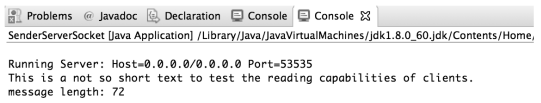
\includegraphics[scale=2.5]{img/sc5.png}
\end{center}
e per il client:
\begin{center}
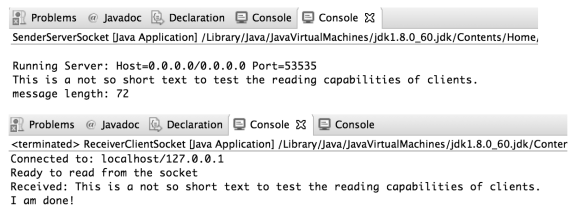
\includegraphics[scale=2.5]{img/sc6.png}
\end{center}
Si nota però che ci sono dei problemi col client, funziona... ma non nella maniera corretta.\\
%pagina 34
\chapter{HTML + CSS + JS}
Innanzitutto una piccola distinzione:
\begin{itemize}
\item un \textbf{linguaggio di programmazione} è utilizzato per comunicare istruzioni a
una macchina di calcolo, per definire programmi che controllino il comportamento di un calcolatore (lo sono \textit{C, Java, C++...})
\item un \textbf{linguaggio di markup} è utilizzato per annotare un documento in modo
tale che l'annotazione sia sintatticamente distinguibile dal testo (lo sono \textit{LaTeX, HTML, XML...}). Qui le annotazioni possono avere diverse finalità:
\begin{itemize}
\item di presentazione (definiscono come visualizzare il testo al quale sono associate)
\item procedurali (definiscono istruzioni per programmi che elaborino il testo al quale sono associate)
\item descrittive (etichettano semplicemente parti del testo, disaccoppiando la struttura dalla presentazione del testo stesso)
\end{itemize}
\end{itemize}
\textbf{HTML} (\textit{Hyper Text Markup Language}) è un linguaggio di markup per dare struttura ai contenuti (web) e la sua specifica è definita dal \textbf{W3C} (\textit{World Wide Web Consortium}). 
\newpage
Vediamo un piccolo esempio:
\begin{center}
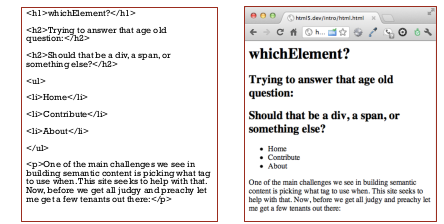
\includegraphics[scale=0.9]{img/html.png}
\end{center}
IL \textbf{CSS} (\textit{Cascading Style Sheets}) è un linguaggio per dare uno stile (di presentazione/visuale) ai contenuti (web) e la sua specifica è definita dal \textbf{W3C} (\textit{World Wide Web Consortium}). 
\\Vediamo un esempio:
\begin{center}
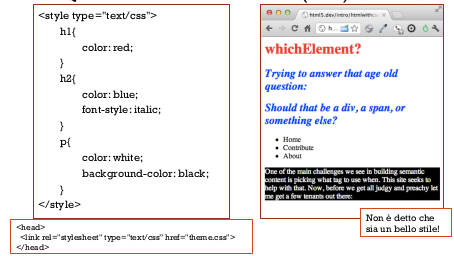
\includegraphics[scale=0.9]{img/css.png}
\end{center}
\begin{center}
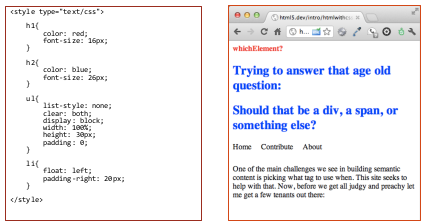
\includegraphics[scale=0.9]{img/css2.png}
\end{center}
Il \textbf{DOM} (\textit{Document Object Model}) è una interfaccia neutrale rispetto al linguaggio di programmazione e alla piattaforma utilizzata per consentire ai programmi l'accesso e la modifica dinamica di contenuto, struttura e stile di un documento (web). \textbf{DOM} è un API definita dal W3C (e implementata da ogni browser moderno) per l'accesso e la gestione dinamica di documenti XML e HTML.\\
Graficamente si ha:
\begin{center}
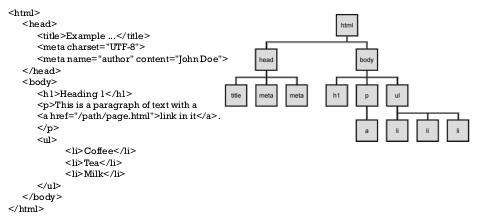
\includegraphics[scale=0.9]{img/dom.png}
\end{center}
\newpage
Ogni nodo può essere caratterizzato da
attributi che ne facilitano l'identificazione, la ricerca, la selezione:
\begin{itemize}
\item un \textbf{identificatore univoco}, anche se il DOM non garantisce l'unicità
\item una \textbf{classe} che indica l'appartenenza ad
un insieme che ci è utile definire
\end{itemize}
Il browser stesso fornisce funzionalità di ricerca, per esempio:
\begin{itemize}
\item \textit{getElementById(IdName)}
\item \textit{getElementsByClassName(ClassName)}
\end{itemize}
\begin{center}
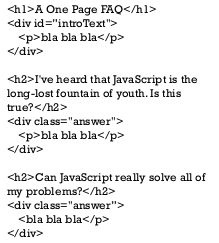
\includegraphics[scale=2.9]{img/dom2.png}
\end{center}
\begin{center}
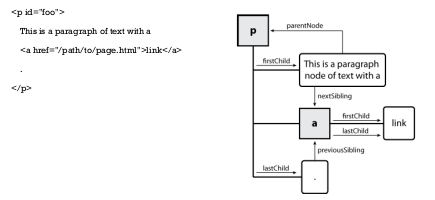
\includegraphics[scale=0.9]{img/dom3.png}
\end{center}
\newpage
Possiamo specificare un selettore più preciso rispetto al
nome del tag, per esempio specificando il nome di una
classe o un identificatore di elemento del DOM:
\begin{minted}{css}
p.intro{
  color:red;
}
\end{minted}
Questo stile sarà applicato solo ai tag di classe intro:
\begin{minted}{html}
<p class = "intro">
\end{minted}
Abbiamo quindi una lista di \textbf{selectors} principali:
\begin{itemize}
\item \textbf{tag name}, il semplice nome del tag:
\begin{minted}{css}
p{
  ...
}
\end{minted}
così quanto scritto si applicherà a tutti i tags <p>
\item il \textbf{dot (.)} applicabile a un tag, indica una classe:
\begin{minted}{css}
p.highlight{
  ...
}
\end{minted}
così quanto scritto si applicherà a tutti i tags <p> con \textit{class =} \textit{"highlight"}
\item lo \textbf{sharp character (\#)}, applicabile a un tag, indica un identificativo:
\begin{minted}{css}
p#intro{
  ...
}
\end{minted}
così quanto scritto si applicherà a tutti i tags <p> con \textit{id = "intro"}
\item i \textbf{two dots (:)} stati comportamentali (ad esempio evento mouseover):
\begin{minted}{css}
p:hover{
  ...
}
\end{minted}
così quanto scritto si applicherà a tutti i tags <p> quando passa sopra il cursore
\item le \textbf{brackets([attr = 'value'])} tag con un valore specifico per un attributo \textit{'value'}:
\begin{minted}{css}
input[type="text"]{
  ...
}
\end{minted}
così quanto scritto si applicherà ai tag di input di tipo \textit{text}
\end{itemize}
Le \textbf{media query} possono essere viste come particolari selettori capaci di valutare le capacità del device di accesso alla pagina (schermi, stamparti, text-to-speech), controllando le dimensioni del device o della finestra, l'orientamento dello schermo e la risoluzione. Vediamo un esempio:\\
\textit{se la pagina è più larga di 480
pixel (e si sta visualizzando sullo schermo), applica
determinati stili agli elementi con id "leftsidebar" (un menu) e "main" (la colonna centrale)}:
\begin{minted}{css}
@media screen and (min-width: 480px){
  #leftsidebar {width: 200px; float: left;}
  #main {margin-left:216px;}
}
\end{minted}
In CSS si ha il termine \textit{cascading} perché esistono potenzialmente diversi stylesheet:
\begin{itemize}
\item l'autore della pagina in genere ne specifica uno (il modo più comunemente inteso) o più d'uno
\item il browser ne ha uno, o un vero e proprio CSS o simulato nel loro codice
\item il lettore, l’utente del browser, ne può definire uno proprio per customizzare la propria esperienza
\end{itemize}
Dei conflitti sono quindi possibili (inevitabili), ed è necessario definire un algoritmo per decidere quale stile vada applicato a un elemento. Si ha il seguente ordine di importanza dei seguenti fattori associati alle regole:
\begin{enumerate}
\item \textbf{importanza} (flag specifico \textit{!important} per un attributo)
\item \textbf{specificità} (per esempio, \textit{id > class > tag})
\item \textbf{ordine nel sorgente }(il più “recente” vince)
\end{enumerate}
Il browser non è solamente un banale visualizzatore di pagine
scritte in HTML, è un vero e proprio ambiente di sviluppo (in
particolare contiene un interprete Javascript e vari strumenti di debug, ma ne parleremo più avanti) che fornisce numerose funzionalità abilitanti inoltre l'impostazione di HTML e CSS separa nettamente il contenuto
dalla modalità di visualizzazione. Esistono numerosi "front-end framework", dai più sofisticati ai
più semplici, naturalmente open
source, ad esempio:
\begin{itemize}
\item \textbf{bootstrap}
\item \textbf{foundation}
\item \textbf{skeleton}
\end{itemize}
\subsubsection{HTML5}
Introduce nuovi \textbf{elementi semantici} per la strutturazione delle pagine, per esempio:
\begin{itemize}
\item article
\item section
\item aside
\item header
\item footer
\end{itemize}
Introduce nuovi \textbf{elementi di input e multimediali}, widget per input search, email, url, number, tel, ma anche range, date... anche se il supporto a tutto ciò da parte dei browser non è uniforme, ma anche audio, video e canvas.\\
Si hanno nuove \textbf{API javascript} per la manipolazione delle pagine: offline data, drag and drop, web storage.\\
quindi si usa:
\begin{itemize}
\item <p> \textit{per definire un paragrafo}
\item <ul> \textit{per definire una lista di elementi il cui ordine non è importante}
\item <address> \textit{per indicare informazioni relative a un indirizzo}
\item <div> e <span> \textit{per contenere informazione che si vuole delimitare per qualche motivo (successive manipolazioni)}
\end{itemize}
Vediamo anche dei brutti usi degli stessi:
\begin{itemize}
\item <p> \textit{per andare a capo}
\item <blockquote> \textit{per gestire l'indentazione}
\item <h1> \textit{per ingrandire del testo}
\end{itemize}
L’HTML dovrebbe non contenere informazione di presentazione, riservata ai CSS, quindi senza stili definiti "in linea" e senza l'uso di tag come <font>, <b>, <i>. \\
Vediamo come sono cambiate le cose con header e footer (quest'ultimo ovviamente con un tag dedicato diverso da quello dell'esempio). \\
Prima:
\begin{minted}{html}
<div id="header">
  <h1>The Awesome Blog of Awesome</h1>
    <p class="tagline">Awesome is a State of Mind</p>
</div>
\end{minted}
poi, con HTML5:
\begin{minted}{html}
<header>
  <h1>The Awesome Blog of Awesome</h1>
  <h2>Awesome is a State of Mind</h2>
</header>
\end{minted}
per i menù di navigazione:\\
Prima:
\begin{minted}{html}
<div id="nav">
  <ul>
    <li><a href="">Home</a></li>
    <li><a href="">Blog</a></li>
    <li><a href="">About</a></li>
    <li><a href="">Contact</a></li>
  </ul>
</div>
\end{minted}
poi, con HTML5:
\begin{minted}{html}
<nav>
  <ul>
    <li><a href="">Home</a></li>
    <li><a href="">Blog</a></li>
    <li><a href="">About</a></li>
    <li><a href="">Contact</a></li>
  </ul>
</nav>
\end{minted}
per articoli.\\
Prima:
\begin{minted}{html}
<div class="post">
  <div class="postheader">
    <h3><a href="">I Scream My Thoughts</a></h3>
    <p class="date">August 10, 2011</p>
  </div> 
  <p>You probably haven't heard of them duis</p>
</div>
\end{minted}
poi, con HTML5:
\begin{minted}{html}
<article>
  <header>
    <h3><a href="">I Scream My Thoughts</a></h3>
    <p class="date">August 10, 2011</p>
  </header> 
  <p>You probably haven't heard of them duis</p>
<article>
\end{minted}
o per i contenuti.\\
Prima:
\begin{minted}{html}
<div class=”content”>
  <div class="post”>
    ...
  </div>
  <div class="post”>
    ...
  </div>
  <div class="post”>
  ...
  </div>
</div>
\end{minted}
poi, con HTML5:
\begin{minted}{html}
<section>
  <article>
    ...
  </article>
  <article>
    ...
  </article>
  <article>
    ...
  <article>
</section>
\end{minted}
Si nota come HTML5 sia più leggibile. In generale, a parte essere una notazione più concisa e che richiede
meno definizioni di classi, le gerarchie di contenuti più leggibili e analizzabili in fase di progettazione, manutenzione e debug.\\
Vediamo un widget per l'input, un widget per il search:
\begin{minted}{html}
<input type=“search” name=“search” />
\end{minted}
\begin{center}
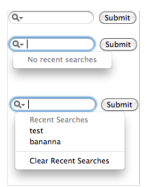
\includegraphics[scale=0.8]{img/see.png}
\end{center}
Questi widget non hanno supporto uniforme e vengono visualizzati diversamente a seconda dei browser ma è supportato da quasi tutti.\\
Vediamo un widget di input per una mail:
\begin{minted}{html}
<input type=“email” name=“email” />
\end{minted}
che fornisce una forma di validazione del dato inserito e forza la tastiera dedicata (con la chiocciola) su device mobili. È supportato da pochissimi browser.
\newpage
Widget per il calendario:
\begin{minted}{html}
<input type=“date” name=“dob” />
\end{minted}
\begin{center}
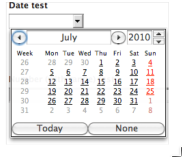
\includegraphics[scale=0.9]{img/date.png}
\end{center}
che fornisce una forma di validazione del dato inserito ma vengono visualizzati diversamente a seconda dei browser ma è supportato da quasi tutti.\\
Manca il modo di definire e governare la dinamicità della pagina, il modo
della pagina di cambiare in modo reattivo al comportamento dell'utente o anche proattivo, senza necessariamente dover attendere uno stimolo dall'utente. Tutto ciò è svolto dal\textbf{ JS}. Il \textbf{Javascript} è il linguaggio di scripting che svolge questa funzione, ne parleremo più avanti in esercitazioni dedicate
\end{document}